\section{Piperchat}

W niniejszym rozdziale zostanie przedstawiona implementacja wideokomunikatora Piperchat. Projekt
składa się z serwera oraz klienta wykonanych w języku Rust. Klient używa także frameworków GTK oraz
GStreamer.

Rysunek \ref{fig:project_tree} prezentuje drzewo projektu.


\begin{figure}[H]
    \centering
    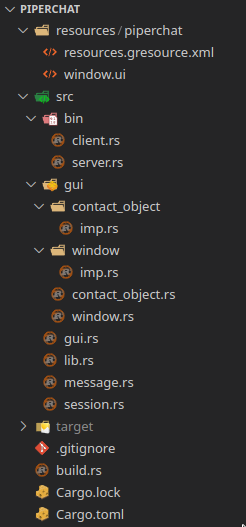
\includegraphics[height=.4\textheight]{img/implementacja/project_tree}
    \caption{Drzewo projektu}
    \label{fig:project_tree}
\end{figure}

\begin{itemize}
    \item \verb|/resources/piperchat| - zawiera pliki XML wykorzystywane przez framework GTK do
          budowy okna
          \begin{itemize}
              \item \verb|resources.gresource.xml| - zawiera listę wszystkich zasobów wykorzystanych w
                    projekcie GTK. W tym wypadku wyliczony jest tylko plik window.ui.
              \item \verb|window.ui| zawiera definicję głównego okna wyrażoną w GTK XML
          \end{itemize}

    \item \verb|/src/| - zawiera cały kod źródłowy w języku Rust
          \begin{itemize}
              \item \verb|/src/bin/| - zawiera pliki źródłowe kompilowane jako osobne programy
                    \begin{itemize}
                        \item \verb|/src/bin/client.rs| - zawiera implementację klienta
                        \item \verb|/src/bin/server.rs| - zawiera implementację serwera
                    \end{itemize}
              \item \verb|/src/lib.rs| - jest punktem wejściowym "biblioteki" tzn. zamieszczone tu
                    elementy są dostępne dla wszystkich programów z katalogu \verb|bin|
              \item \verb|/src/message.rs| - zawiera definicje wiadomości wysyłanych pomiędzy
                    klientem a serwerem.
              \item \verb|/src/gui.rs| - definiuje moduł \verb|gui| składający się z modułów
                    \verb|window| oraz \verb|contact_object|
                    \begin{itemize}
                        \item \verb|/src/gui/window.rs| - zawiera definicję okna aplikacji jako
                              obiektu GTK
                              \begin{itemize}
                                  \item \verb|/src/gui/window/imp.rs| - zawiera implementację okna
                                        aplikacji jako obiektu GTK
                              \end{itemize}
                        \item \verb|/src/gui/contact_object.rs| - zawiera definicję kontaktu (tj. innego
                              połączonego i dostępnego użytkownika) jako obiektu GTK
                              \begin{itemize}
                                  \item \verb|/src/gui/contact_object/imp.rs| - zawiera
                                        implementację kontaktu jako obiektu GTK
                              \end{itemize}
                    \end{itemize}
          \end{itemize}

    \item \verb|build.rs| zawiera skrypt budujący zasoby z katalogu \verb|resources|
    \item \verb|Cargo.toml| zawiera manifest projektu Rust wraz z listą bezpośrednich
          zależności
    \item \verb|Cargo.lock| lockfile zawierający wyznaczone wersje wszystkich zainstalowanych
          zależności
\end{itemize}

\subsection{Serwer}

Do komunikacji wykorzystywane są protokoły TCP i WebSockets. TCP zapewnia gwarancję poprawności
odebranych danych i ich odpowiedniej kolejności, zamienia strumień pakietów na łańcuch bajtów
przychodzący w kolejności. Protokół Websockets zapewnia framing, czyli zamienia łańcuch bajtów na
strumień wiadomości które mogą mieć różną wielkość i zawierać dane tekstowe lub binarne. Protokół
aplikacji wykorzystuje tylko dane tekstowe.

\subsubsection{Protokół aplikacji}

Rodzaje komunikatów możliwych do wysłania przez klient lub serwer są zebrane w odpowiedni typ
wyliczeniowy a następnie w wiadomości tekstowej Websockets wysyłana jest ich serializacja w formacie
JSON (ang. Javascript Object Notation).

\begin{minted}{rust}
use serde::{Deserialize, Serialize};

#[derive(Serialize, Deserialize, Debug, Clone)]
#[serde(rename_all = "lowercase")]
pub enum Message {
    Connect(ConnectMessage),
    ConnectResponse(ConnectResponse),
    UserList(UserList),
    Webrtc(WebrtcMsg),
    Call(CallMessage),
    CallReceived(CallReceivedMessage),
    CallHangup,
    CallResponse(CallResponseMessage),
}
\end{minted}

Implementacja serwera wykorzystuje dwie techniki komunikacji wieloprocesowej:

\begin{itemize}
    \item synchronizacja dostępu do dzielonych danych
    \item przekazywanie wiadomości
\end{itemize}

Diagram \ref{fig:server_data_flow} prezentuje wysokopoziomową strukturę działania serwera: dla
każdego połączenia uruchamiane jest nowe zadanie które zajmuje się komunikacją z danym socketem.
Wraz z zadaniami tworzone są kanały służące do wysyłania komend przez resztę systemu dla danego
połączenia. Gdy rozpoczyna się nowe połączenie pomiędzy użytkownikami X i Y, zadanie użytkownika X
otrzymuje wysyłacz komend do użytkownika Y i vice versa. Zadanie na wiadomości otrzymane od
użytkownika reaguje wysyłając komendy przez wysyłacz do drugiej strony połączenia, a na otrzymane
przez swój własny słuchacz komendy może reagować wysyłając wiadomości na swój socket.

\begin{figure}[H]
    \centering
    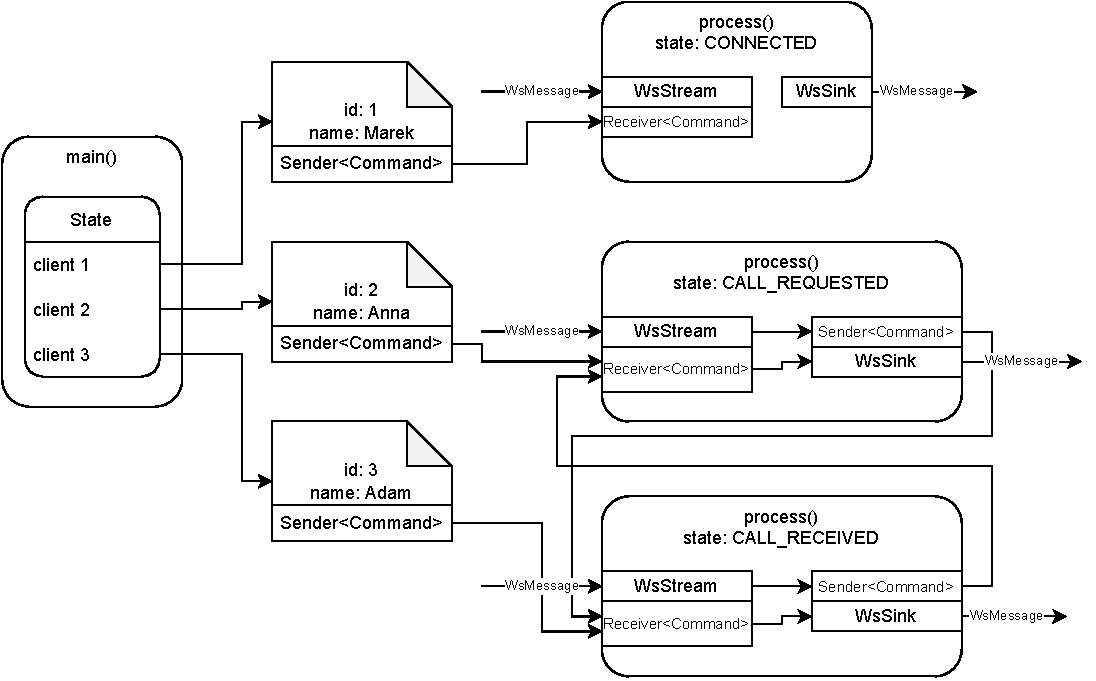
\includegraphics[width=0.9\textwidth]{img/implementacja/server_data_flow}
    \caption{Diagram przepływu danych serwera}
    \label{fig:server_data_flow}
\end{figure}

\subsubsection{Fragmenty kodu}

\paragraph{Główna pętla}

\begin{listing}[H]
    \begin{minted}{rust}

#[tokio::main]
async fn main() -> color_eyre::Result<()> {
    pretty_env_logger::init();
    color_eyre::install()?;
    let listener = TcpListener::bind("0.0.0.0:2137").await.unwrap();
    let state = Arc::new(Mutex::new(State::new()));

    loop {
        let (socket, _) = listener.accept().await.unwrap();
        let state = state.clone();
        tokio::spawn(async move { process(socket, state).await.unwrap() });
    }
}
    \end{minted}
    \caption{Główna pętla serwera akceptująca przychodzące połączenia TCP}
    \label{lst:server_main_loop}
\end{listing}

Listing \ref{lst:server_main_loop} zawiera funkcję \verb|main| serwera, która najpierw inicjalizuje
handlery systemu logów oraz raportowania błędów, inicjalizuje obiekt \verb|TcpListener|, a
także globalny stan aplikacji który zawiera listę aktualnie połączonych użytkowników. Obiekt
\verb|State|, którego definicja znajduje się w listingu \ref{lst:server_state}, synchronizowany jest
pomiędzy wątkami za pomocą muteksu, a następnie muteks pakowany jest w \verb|Arc| (Atomic Reference
Counter), który jest odpowiednikiem \verb|std::shared_ptr| z C++ i odpowiada za dzielenie muteksu
pomiędzy wątki oraz zwolnienie go gdy liczba żyjących referencji osiągnie 0.

Dzięki użyciu atrybutu \verb|tokio::main|, funkcja main jest asynchroniczna i można w
niej korzystać z \verb|.await|.

\begin{listing}[H]
    \begin{minted}{rust}
struct State {
    users: HashMap<u32, User>,
}

impl State {
    fn new() -> Self {
        State {
            users: HashMap::new(),
        }
    }
}

#[derive(Debug)]
struct User {
    name: String,
    id: u32,
    tx: mpsc::UnboundedSender<Command>,
}
    \end{minted}
    \caption{Obiekt State zawierający globalny stan serwera}
    \label{lst:server_state}
\end{listing}

\paragraph{Funkcja process}

Funkcja process odpowiedzialna jest za komunikację z każdym z klientów. Wykonuje następujące
zadania:

\begin{enumerate}
    \item Otrzymuje wiadomość \verb|Connect| od klienta
    \item Dodaje klienta do obiektu State
    \item Przechowuje aktualny stan klienta (połączony/wysłał lub otrzymał połączenie/w połączeniu,
          etc.)
    \item Za pomocą makra \verb|select!| nasłuchuje na jedno z możliwych wydarzeń:
          \begin{itemize}
              \item Wiadomość przychodząca od użytkownika
              \item Komenda przychodząca przez kanał
          \end{itemize}
    \item Po rozłączeniu, usunięcie z listy użytkowników w obiekcie \verb|State|.
\end{enumerate}

\paragraph{Stan użytkownika}

Algebraiczne typy danych dostępne w języku Rust znacząco ułatwiają modelowanie stanu programu.
Oprócz \emph{product types} dostępnych w także innych językach programowania jako struktury
(ponieważ liczba wszystkich możliwych wartości struktury to iloczyn wartości jej pól), mamy także
dostęp do \emph{sum types} realizowanych poprzez pola wyliczeniowe \verb|enum|, które dodatkowo mogą
zawierać dane. W takim wypadku suma wszystkich możliwych wartości pola wyliczeniowego jest sumą
wartości jego wariantów.

\begin{listing}[H]
    \begin{minted}{rust}
#[derive(Debug)]
enum ClientState {
    Connected,
    CallRequested(mpsc::UnboundedSender<Command>),
    CallReceived(mpsc::UnboundedSender<Command>),
    InCall(mpsc::UnboundedSender<Command>),
}
    \end{minted}
    \caption{Pole wyliczeniowe możliwych stanów klienta}
    \label{lst:server_client_state}
\end{listing}

Listing \ref{lst:server_client_state} zawiera pole wyliczeniowe \verb|ClientState|, które w
wariantach Call może zawierać obiekt \verb|UnboundedSender|, który służy do wysyłania wiadomości
typu \verb|Command| (listing \ref{lst:server_command}) do odbiorników które znajdują się w innych
klientach. W ten sposób odbywa się komunikacja pomiędzy klientami.

\begin{listing}[H]
    \begin{minted}{rust}
#[derive(Debug)]
enum Command {
    SendMessage(PcMessage),
    CallReceived {
        channel: mpsc::UnboundedSender<Command>,
        name: String,
    },
    CallAccepted(mpsc::UnboundedSender<Command>),
    PeerHungup,
    CallRejected,
}
    \end{minted}
    \caption{Komendy możliwe do wysłania przez jednego klienta do drugiego}
    \label{lst:server_command}
\end{listing}



\subsection{Klient}

Aplikacja okienkowa składa się z czterech konkurentnie wykonujących się zadań:

\begin{enumerate}
    \item Zadanie GUI, rysuje okienko oraz emituje zdarzenia GUI
    \item Zadanie połączenia z serwerem, nasłuchuje wiadomości wysłane przez serwer, emituje
          zdarzenia sieciowe, odbiera komendy do wykonania
    \item Zadanie połączenia, prowadzi proces sygnalizacji i negocjacji WebRTC, a następnie prowadzi
          połączenie: prezentuje strumienie audio-wideo użytkownikowi oraz wysyła strumienie wideo i
          audio drugiej stronie połączenia. Działa od rozpoczęcia połączenia do jego zakończenia.
          Bardzo ograniczona komunikacja z zadaniem głównym.
\end{enumerate}

Rdzeń aplikacji odpowiedzialny jest za odbieranie zdarzeń od zadań i reagowanie na nie wysyłając
komendy do innych zadań. Np. odbieranie zdarzenia kliknięcia w przycisk rozpoczęcia połączenia
obok użytkownika X powoduje wysłanie komendy "zadzwoń do użytkownika X" do zadania połączenia.
Podobnie gdy zadanie połączenia odbierze od serwera wiadomość \verb|UserList|, rdzeń odbiera to
zdarzenie i wysyła komendę do zadania GUI by zaktualizowało listę dostępnych użytkowników.

Wyjątkiem jest zadanie GStreamer które komunikuje się bezpośrednio z zadaniem połączenia. Powody
takiej decyzji są dwa:

\begin{itemize}
    \item Zadanie GStreamer wysyła i odbiera dużą ilość danych które nie mają żadnego efektu w GUI,
          więc bezpośrednie połączenie sprawia że rdzeń nie musi być ich świadom
    \item Dopóki trwa rozmowa, użytkownik nie może rozpoczynać ani odbierać żadnych nowych rozmów
\end{itemize}

Diagram \ref{fig:client_data_flow} obrazuje wysokopoziomową strukturę danych klienta. Główna funkcja
aplikacji tworzy zadania do obsługi interfejsu graficznego (GUI task) oraz do obsługi połączenia z
serwerem aplikacji (Network task). Komunikacja pomiędzy zadaniami odbywa się poprzez wysyłanie
silnie typowanych wiadomości przez specjalne kanały. Obiekt \verb|EventHandler| jednocześnie
nasłuchuje na zdarzenia \verb|GuiEvent| od zadania GUI oraz zdarzenia \verb|NetworkEvent| od zadania
połączenia, następnie reaguje na nie wykonując operacje na lub wysyłając komendy do tego drugiego.

\begin{figure}[H]
    \centering
    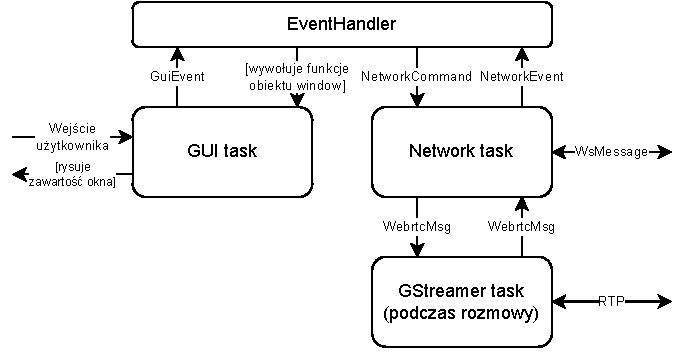
\includegraphics[width=0.9\textwidth]{img/implementacja/client_data_flow}
    \caption{Diagram przepływu danych klienta}
    \label{fig:client_data_flow}
\end{figure}

\subsubsection{EventHandler}

Obiekt \verb|EventHandler| zajmuje się reagowaniem na zdarzenia z obu zadań. Listing
\ref{lst:eventhandler} zawiera definicję obiektu oraz zawartość funkcji \verb|start|, która
uruchamia proces handlowania zdarzeń. Obiekt nasłuchuje na przychodzące zdarzenia, a następnie
obsługuje je w osobnych funkcjach, które zostaną omówione w czasie omawiania poszczególnych zadań.

\begin{minted}{rust}
struct EventHandler {
    gui_rx: Receiver<GuiEvent>,
    network_rx: Receiver<NetworkEvent>,
    network_command_tx: Sender<NetworkCommand>,
    current_dialog: Option<MessageDialog>,
    window: Window,
}

impl EventHandler {
    fn start(mut self) {
        let event_handler = async move {
            loop {
                select! {
                    network_event = self.network_rx.next() => {
                        match network_event {
                            Some(event) => self.handle_network_event(event).await,
                            None => break
                        }
                    },
                    gui_event = self.gui_rx.next() => {
                        match gui_event {
                            Some(event) => self.handle_gui_event(event).await,
                            None => break
                        }
                    }
                }
            }
        };

        MainContext::default().spawn_local(event_handler);
    }
    ...
}
\end{minted}
\captionof{listing}{Definicja obiektu EventHandler oraz jego metody obsługującej zdarzenia\label{lst:eventhandler}}

\subsubsection{Zadanie GUI}

GUI emituje następujące zdarzenia (listing \ref{lst:guievent}):

\begin{listing}[H]
    \begin{minted}{rust}
#[derive(Debug)]
pub enum GuiEvent {
    CallStart(u32, String),
    CallAccepted(VideoPreference),
    CallRejected,
    NameEntered(String),
}
\end{minted}
    \caption{Definicja pola wyliczeniowego GuiEvent}
    \label{lst:guievent}
\end{listing}

Są one obsługiwane w następujący sposób (listing \ref{lst:guievent_handler}):

\begin{minted}{rust}
async fn handle_gui_event(&mut self, event: GuiEvent) {
    match event {
        GuiEvent::CallStart(id, name) => {
            let dialog = adw::MessageDialog::new(
                Some(&self.window),
                Some(&format!("Calling {name}")),
                Some(&format!(
                "Waiting for a response from {name}. You can wait for the answer or hangup."
            )),
            );
            dialog.add_responses(&[("hangup", "Hang up")]);
            dialog.set_response_appearance("hangup", ResponseAppearance::Destructive);

            let network_command_tx = self.network_command_tx.clone();
            dialog.run_async(None, move |obj, response| {
                if response == "hangup" {
                    info!("SENDING HANGUP");
                    network_command_tx
                        .send_blocking(NetworkCommand::CallHangup)
                        .unwrap();
                }
            });
            self.current_dialog = Some(dialog);

            self.network_command_tx
                .send_blocking(NetworkCommand::CallStart(id, name))
                .unwrap();
        }
        GuiEvent::CallAccepted(preference) => {
            self.network_command_tx
                .send_blocking(NetworkCommand::CallAccept)
                .unwrap();
        }

        GuiEvent::CallRejected => {
            self.network_command_tx
                .send_blocking(NetworkCommand::CallReject)
                .unwrap();
        }
        GuiEvent::NameEntered(name) => {
            self.network_command_tx
                .send_blocking(NetworkCommand::Connect(name))
                .unwrap();
        }
    }
}
\end{minted}
\captionof{listing}{Metoda obsługująca zdarzenia GuiEvent\label{lst:guievent_handler}}

\subsubsection{Zadanie połączenia}

Zadanie połączenia emituje następujące zdarzenia (listing \ref{lst:networkevent}):

\begin{listing}[H]
    \begin{minted}{rust}
#[derive(Debug)]
pub enum NetworkEvent {
    UserlistReceived(Vec<(u32, String)>),
    CallReceived(String),
    CallAccepted,
    CallRejected(String),
    CallHangup(String),
}
\end{minted}
    \caption{Definicja pola wyliczeniowego NetworkEvent}
    \label{lst:networkevent}
\end{listing}

oraz akceptuje następujące komendy (listing \ref{lst:networkcommand}):

\begin{listing}[H]
    \begin{minted}{rust}
#[derive(Debug)]
pub enum NetworkCommand {
    CallStart(u32, String),
    CallAccept,
    CallReject,
    CallHangup,
    Connect(String),
}
\end{minted}
    \caption{Definicja pola wyliczeniowego NetworkCommand}
    \label{lst:networkcommand}
\end{listing}

Zdarzenia sieciowe są obsługiwane w następujący sposób:

\begin{minted}{rust}
async fn handle_network_event(&mut self, event: NetworkEvent) {
    info!("received network event: {event:?}");
    match event {
        NetworkEvent::UserlistReceived(userlist) => {
            self.window.set_contacts(userlist);
        }
        NetworkEvent::CallReceived(name) => {
            // display a dialog where user can accept/reject the message
            let dialog = adw::MessageDialog::new(
                Some(&self.window),
                Some(&format!("Incoming call from {name}")),
                Some(&format!(
                    "Receiving a call from {name}. Do you want to accept or reject this call?"
                )),
            );
            dialog.add_responses(&[("accept", "Accept"), ("reject", "Reject")]);
            dialog.set_response_appearance("accept", ResponseAppearance::Suggested);
            dialog.set_response_appearance("reject", ResponseAppearance::Destructive);
            let window = self.window.clone();

            dialog.run_async(None, move |_obj, response| match response {
                "accept" => {
                    window.accept_call();
                }
                "reject" => {
                    window.reject_call();
                }
                // here dialog got closed from outside, that means sender hung up
                _ => {
                    let dialog = adw::MessageDialog::new(
                        Some(&window),
                        Some(&format!("Caller hung up.")),
                        Some(&format!(
                            "The call from the user {name} terminated. Caller hung up."
                        )),
                    );

                    dialog.add_responses(&[("ok", "OK")]);
                    dialog.run_async(None, move |obj, response| {});
                }
            });
            self.current_dialog = Some(dialog);
        }
        NetworkEvent::CallHangup(name) => {
            info!("Received hangup");
            if let Some(dialog) = self.current_dialog.take() {
                dialog.close();
            }
        }
        NetworkEvent::CallAccepted => {
            if let Some(dialog) = self.current_dialog.take() {
                info!("CLOSING");
                dialog.close();
            }
        }
        NetworkEvent::CallRejected(name) => {
            if let Some(dialog) = self.current_dialog.take() {
                info!("CLOSING");
                dialog.close();
            }

            let dialog = adw::MessageDialog::new(
                Some(&self.window),
                Some(&format!("Call rejected")),
                Some(&format!("Recepient {name} rejected the call.")),
            );

            dialog.add_responses(&[("ok", "OK")]);
            dialog.run_async(None, move |obj, response| {});
        }
    }
}
\end{minted}
\captionof{listing}{Metoda obsługująca zdarzenia NetworkEvent\label{lst:networkevent_handler}}

\subsubsection{Zadanie GStreamer}

Zadanie GStreamer jest tworzone gdy rozpoczynane jest nowe połączenie, i jest niszczone gdy
połączenie jest zamykane.

\paragraph{Pipeline}

W konstruktorze obiektu z reprezentacji tekstowej tworzony jest pipeline kierujący lokalne
strumienie wideo i audio do elementu webrtcbin (listing \ref{lst:pipeline-1}):

\begin{listing}[H]
    \begin{minted}{rust}
// Create the GStreamer pipeline
let pipeline = gst::parse_launch(
    "v4l2src ! videoconvert ! vp8enc deadline=1 ! rtpvp8pay pt=96 ! webrtcbin. \
    autoaudiosrc ! opusenc ! rtpopuspay pt=97 ! webrtcbin. \
    webrtcbin name=webrtcbin",
)?;
\end{minted}
    \caption{Reprezentacja tekstowa pipeline'u}
    \label{lst:pipeline-1}
\end{listing}

Następnie do pipeline'u dołączane są zdalne strumienie mediów pojawiające się za pomocą sygnału
\verb|pad_added|. Przychodzące strumienie muszą najpierw zostać odkodowane za pomocą elementu
decodebin (listing \ref{lst:pipeline-2}):

\begin{minted}{rust}
app.webrtcbin.connect_pad_added(move |_webrtc, pad| {
    let app = upgrade_weak!(app_clone);

    if let Err(err) = app.on_incoming_stream(pad) {
        gst::element_error!(
            app.pipeline,
            gst::LibraryError::Failed,
            ("Failed to handle incoming stream: {:?}", err)
        );
    }
});

...

// Whenever there's a new incoming, encoded stream from the peer create a new decodebin
fn on_incoming_stream(&self, pad: &gst::Pad) -> Result<(), anyhow::Error> {
    // Early return for the source pads we're adding ourselves
    if pad.direction() != gst::PadDirection::Src {
        return Ok(());
    }

    let decodebin = gst::ElementFactory::make("decodebin").build().unwrap();
    let app_clone = self.downgrade();
    decodebin.connect_pad_added(move |_decodebin, pad| {
        let app = upgrade_weak!(app_clone);

        if let Err(err) = app.on_incoming_decodebin_stream(pad) {
            gst::element_error!(
                app.pipeline,
                gst::LibraryError::Failed,
                ("Failed to handle decoded stream: {:?}", err)
            );
        }
    });

    self.pipeline.add(&decodebin).unwrap();
    decodebin.sync_state_with_parent().unwrap();

    let sinkpad = decodebin.static_pad("sink").unwrap();
    pad.link(&sinkpad).unwrap();

    Ok(())
}
\end{minted}
\captionof{listing}{Dekodowanie zdalnych strumieni\label{lst:pipeline-2}}

Następnie zdekodowane strumienie są dodawane do pipeline'u w funkcji
\verb|on_incoming_decodebin_stream(pad)| (listing \ref{lst:pipeline-3}):

\begin{listing}[H]
    \begin{minted}{rust}
// Handle a newly decoded decodebin stream and depending on its type, create the relevant
// elements or simply ignore it
fn on_incoming_decodebin_stream(&self, pad: &gst::Pad) -> Result<(), anyhow::Error> {
    let caps = pad.current_caps().unwrap();
    let name = caps.structure(0).unwrap().name();

    let sink = if name.starts_with("video/") {
        gst::parse_bin_from_description(
            "queue ! videoconvert ! videoscale ! autovideosink",
            true,
        )?
    } else if name.starts_with("audio/") {
        gst::parse_bin_from_description(
            "queue ! audioconvert ! audioresample ! autoaudiosink",
            true,
        )?
    } else {
        println!("Unknown pad {:?}, ignoring", pad);
        return Ok(());
    };

    self.pipeline.add(&sink).unwrap();
    sink.sync_state_with_parent()
        .with_context(|| format!("can't start sink for stream {:?}", caps))?;

    let sinkpad = sink.static_pad("sink").unwrap();
    pad.link(&sinkpad)
        .with_context(|| format!("can't link sink for stream {:?}", caps))?;

    Ok(())
}
\end{minted}
    \caption{Dodawanie zdekodowanych strumieni do pipeline'u}
    \label{lst:pipeline-3}
\end{listing}


\subsubsection{Interfejs użytkownika}

W niniejszym rozdziale zaprezentowany zostanie interfejs użytkownika wykonany za pomocą frameworka
GTK oraz biblioteki libadwaita.

Po uruchomieniu aplikacji prezentowany jest ekran lądowania który wyświetla wiadomość powitalną oraz
prosi o podanie nazwy użytkownika (rys. \ref{fig:screen_landing}).

\begin{figure}[H]
    \centering
    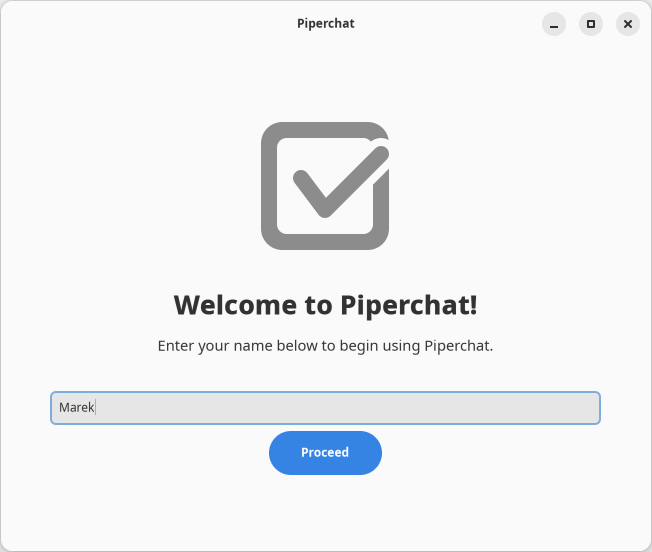
\includegraphics[width=.5\textwidth]{img/gui/screen_landing}
    \caption{Ekran lądowania}
    \label{fig:screen_landing}
\end{figure}

Po wprowadzeniu nazwy użytkownika aplikacja łączy się z serwerem, ogłasza dostępność użytkownika
innym połączonym użytkownikom oraz wyświetla użytkownikowi listę innych połączonych użytkowników
(rys. \ref{fig:screen_main}).

\begin{figure}[H]
    \centering
    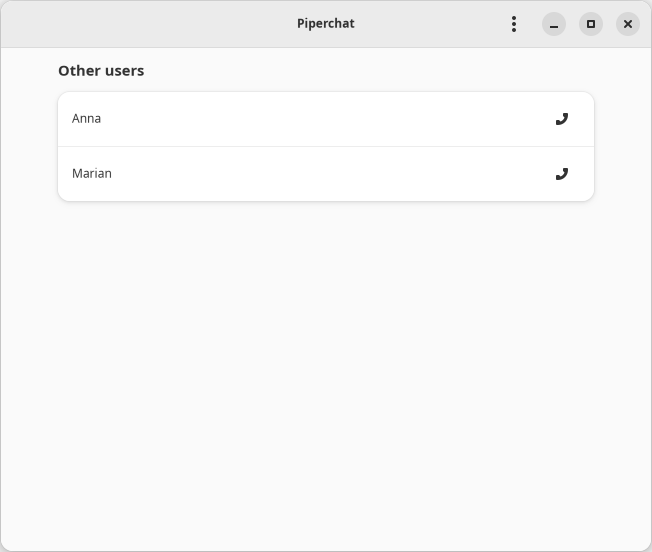
\includegraphics[width=.5\textwidth]{img/gui/screen_main}
    \caption{Główny ekran aplikacji}
    \label{fig:screen_main}
\end{figure}

Użytkownik może zadzwonić do drugiego użytkownika klikając na przycisk rozpoczęcia połączenia po
prawej stronie nazwy innego użytkownika. Podczas oczekiwania na odpowiedź od odbiorcy, wyświetlane
jest następujące okno dialogowe, gdzie nadawca może przerwać połączenie (rys.
\ref{fig:screen_call_start}):

\begin{figure}[H]
    \centering
    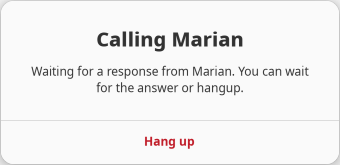
\includegraphics[width=.5\textwidth]{img/gui/screen_call_start}
    \caption{Dialog wysłania połączenia}
    \label{fig:screen_call_start}
\end{figure}

Tymczasem odbiorcy prezentowane jest okno dialogowe informujące o przychodzącym połączeniu. Odbiorca
może odebrać lub odrzucić połączenie (rys. \ref{fig:screen_call_recv}):

\begin{figure}[H]
    \centering
    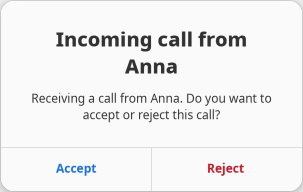
\includegraphics[width=.4\textwidth]{img/gui/screen_call_recv}
    \caption{Dialog otrzymania połączenia}
    \label{fig:screen_call_recv}
\end{figure}

Jeżeli odbiorca odrzuci połączenie, nadawcy wyświetla się okno dialogowe informujące o zdarzeniu
(rys. \ref{fig:screen_recepient_reject}):

\begin{figure}[H]
    \centering
    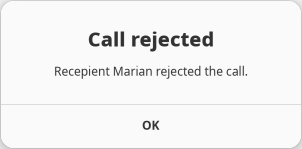
\includegraphics[width=.4\textwidth]{img/gui/screen_recepient_reject}
    \caption{Dialog odrzucenia połączenia przez odbiorcę}
    \label{fig:screen_recepient_reject}
\end{figure}

Jeżeli połączenie zostanie przerwane przez nadawcę zanim nadawca zdąży odebrać albo odrzucić
połączenie, okno dialogowe informujące o zdarzeniu wyświetlane jest odbiorcy (rys. \ref{fig:screen_caller_hungup}):

\begin{figure}[H]
    \centering
    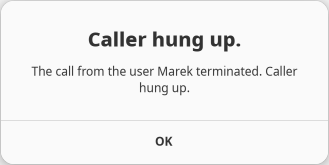
\includegraphics[width=.4\textwidth]{img/gui/screen_caller_hungup}
    \caption{Dialog porzucenia połączenia przez nadawcę}
    \label{fig:screen_caller_hungup}
\end{figure}
